\documentclass{article}
\usepackage[utf8]{inputenc}
\usepackage{lmodern}
\usepackage{amsmath}
\usepackage{parskip}
\usepackage[hyphens]{url}
\usepackage{graphicx}
\graphicspath{{./}}
\setlength{\skip\footins}{1cm}
\newcommand{\code}[1]{\colorbox{gray}{\texttt{#1}}}
\title{Hal\_3900 Proposal}
\begin{document}
\begin{LARGE}
\begin{center}
\vspace*{15mm}

COMP3900

Hal\_3900 Report

\rule[4.5pt]{0.8\textwidth}{0.3pt}

\begin{align*}
  \text{Ellen Oates}  \quad &\text{z5098896 \enspace Developer} \\
  \text{Hayden Le}    \quad &\text{z5098972 \enspace Developer} \\
  \text{Yi Wang}      \quad &\text{z5124282 \enspace Developer} \\
  \text{Zain Afzal}   \quad &\text{z5059449 \enspace Scrum Master}
\end{align*}

\vspace*{8mm}
\rule[4.5pt]{0.8\textwidth}{0.3pt}

08/03/2019

\end{center}
\end{LARGE}

\vfill
\small{e.l.oates@unsw.edu.au}\\
\small{hayden.le@unsw.edu.au}\\
\small{z.afzal@unsw.edu.au}\\
\small{yi.wang7@student.unsw.edu.au}

\newpage
\tableofcontents 

%-------------------------------------------------------------------------------------------------%

\newpage
\section{Introduction}

\subsection{The Problem}
Online learning is changing the way students access and engage with higher education. Courses with online delivery increase the flexibility and accessibility of education by providing students with a platform to learn course content in their own time, at their own pace. Increasingly courses which are taught face to face include some online content delivery, including course materials, quizzes, online lecture recordings, and forums to ask questions and discuss the course content outside of class. Because online learning is so prevalent in higher education, it is crucial for universities to ensure students are satisfied with their learning experience. 

There is a delay between when students ask a question and when they get a response, and this can vary from hours to days. Answering individual student questions via email or on forums requires a significant amount of time for tutors, course administrators and lecturers. Often the same questions will be asked many times by different students, making it inefficient to have course staff respond to each one individually.

Some key factors that contribute to student satisfaction in the online learning space are:
\begin{itemize}
  \item Students' preferences for actively participating in learning, rather than through passive learning styles.
  \item Students' expectations on instructors to facilitate their learning by organising the course resources\footnote{\url{https://www.researchgate.net/publication/282699144_Student_Satisfaction_with_Online_Learning_Is_it_a_Psychological_Contract}}
  \item The amount of interaction students have with each other, and the availability of their instructors.\footnote{'Key Factors for Determining Student Satisfaction in Online Courses': \url{https://www.learntechlib.org/primary/p/2226/article_2226.pdf}}
  \item The availability of strong administrative support when using online learning tools or when confused about assessments and learning expectations.
  \item Course staff who are concerned with the quality of their course delivery, and want to know what their students need the most help with
  \item The availability of individual support and extended materials
\end{itemize}

Making these factors available to students becomes more challenging as classes grow in size. Course staff are thus in need of a more effective way to support with their students. 

\subsection{Existing Solutions \& Problems}

Currently at UNSW, learning support is provided to students through email, forums and help sessions. This is very man-hour intensive, requiring many tutors to be on hand to answer questions which, of themselves, are quite repetitive. In addition, as these courses become larger with increasing enrollment sizes, it becomes more difficult to be able to give students individual attention.

Another side effect of growing cohort sizes is the fact that many tutors and lecturers are forced to spend most of their time answering admin related questions, which is time that could be spent improving the course. The current solution has been to hire more staff and offload the majority of questions to forums, however these are full of repeated questions and require many tutors to moderate them.

This growth is becoming unsustainable, and with the rise of online education platforms, many students are eager to interact with course material in a more meaningful way. Waiting for a tutor to respond often creates a disconnect between the initial question and the answer, which limits the effectiveness of the response. This is provided that the tutor finds time to respond at all.

Chat bots have been deployed in some areas of secondary education, which interact with students in meaningful ways outside of class hours\footnote{\url{https://botsify.com/education-chatbot}}, and some have even been created to answer university-level questions\footnote{\url{https://www.canberra.edu.au/about-uc/media/newsroom/2018/february/students-make-new-friend-in-lucy-the-chatbot}}. However these tools can not be easily adopted by all university courses, or their administration and assessments.

\subsection{Our Solution}

\subsubsection{Our Contributions}

\subsubsection{Aim \& Purpose}

\subsubsection{Differences to Existing Systems}
% Why is our system better?
% What are the innovative points of our system compared to existing ones?


\newpage
\section{Background}

\subsection{Usage Scenario}
% Example domain
% Who are the users of the system?
% How does the system process the users' requests?

\subsection{System Architecture}

\subsubsection{Architecture Diagram}
%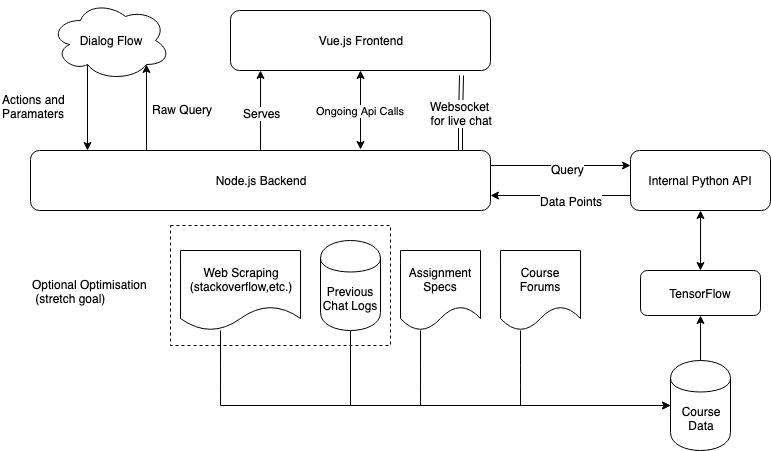
\includegraphics[width=\textwidth]{architecture_diagram.png}

\subsubsection{Data Scraping \& Processing}

\subsubsection{Extensible API}

\subsubsection{Interactive User Interface}


\newpage
\section{Data Scraping \& Processing}

\subsection{Input \& Output}
% describe input & output
% what happens after receiving input
% how does it produce the output

\subsection{Example Usage}
% include 1-2 screenshots

\subsection{Technical Details}
% refer to appendix


\newpage
\section{Extensible API}

\subsection{Input \& Output}
% describe input & output
% what happens after receiving input
% how does it produce the output

\subsection{Example Usage}
% include 1-2 screenshots

\subsection{Technical Details}
% refer to appendix


\newpage
\section{Interactive User Interface}

\subsection{Input \& Output}
% describe input & output
% what happens after receiving input
% how does it produce the output

\subsection{Example Usage}
% include 1-2 screenshots

\subsection{Technical Details}
% refer to appendix


\newpage
\section{Conclusion}

\subsection{How Existing Problems Were Addressed}

\subsection{Improvements}

\newpage
\section{Appendix}

\subsection{Technologies}

\subsubsection{Node.js}

\subsubsection{Vue.js}

\subsubsection{Dialogflow}

\subsubsection{Google NLP}

\end{document}
